\documentclass{article}
\usepackage[most]{tcolorbox}
\usepackage{tikz}
\usepackage[margin=0.1in]{geometry}
\begin{document}
\centering\textbf{CoCoSci NIPS Data Blitz!}

Draw diagrams, sometimes on a grid. You can draw rectangles, lines, arrows,
dashed lines, and circles of radius 1 grid cell.  Your drawings don't have to be
perfect, but they should be good enough for a human to understand. On
the last grid you can draw whatever diagram you want.

\centering
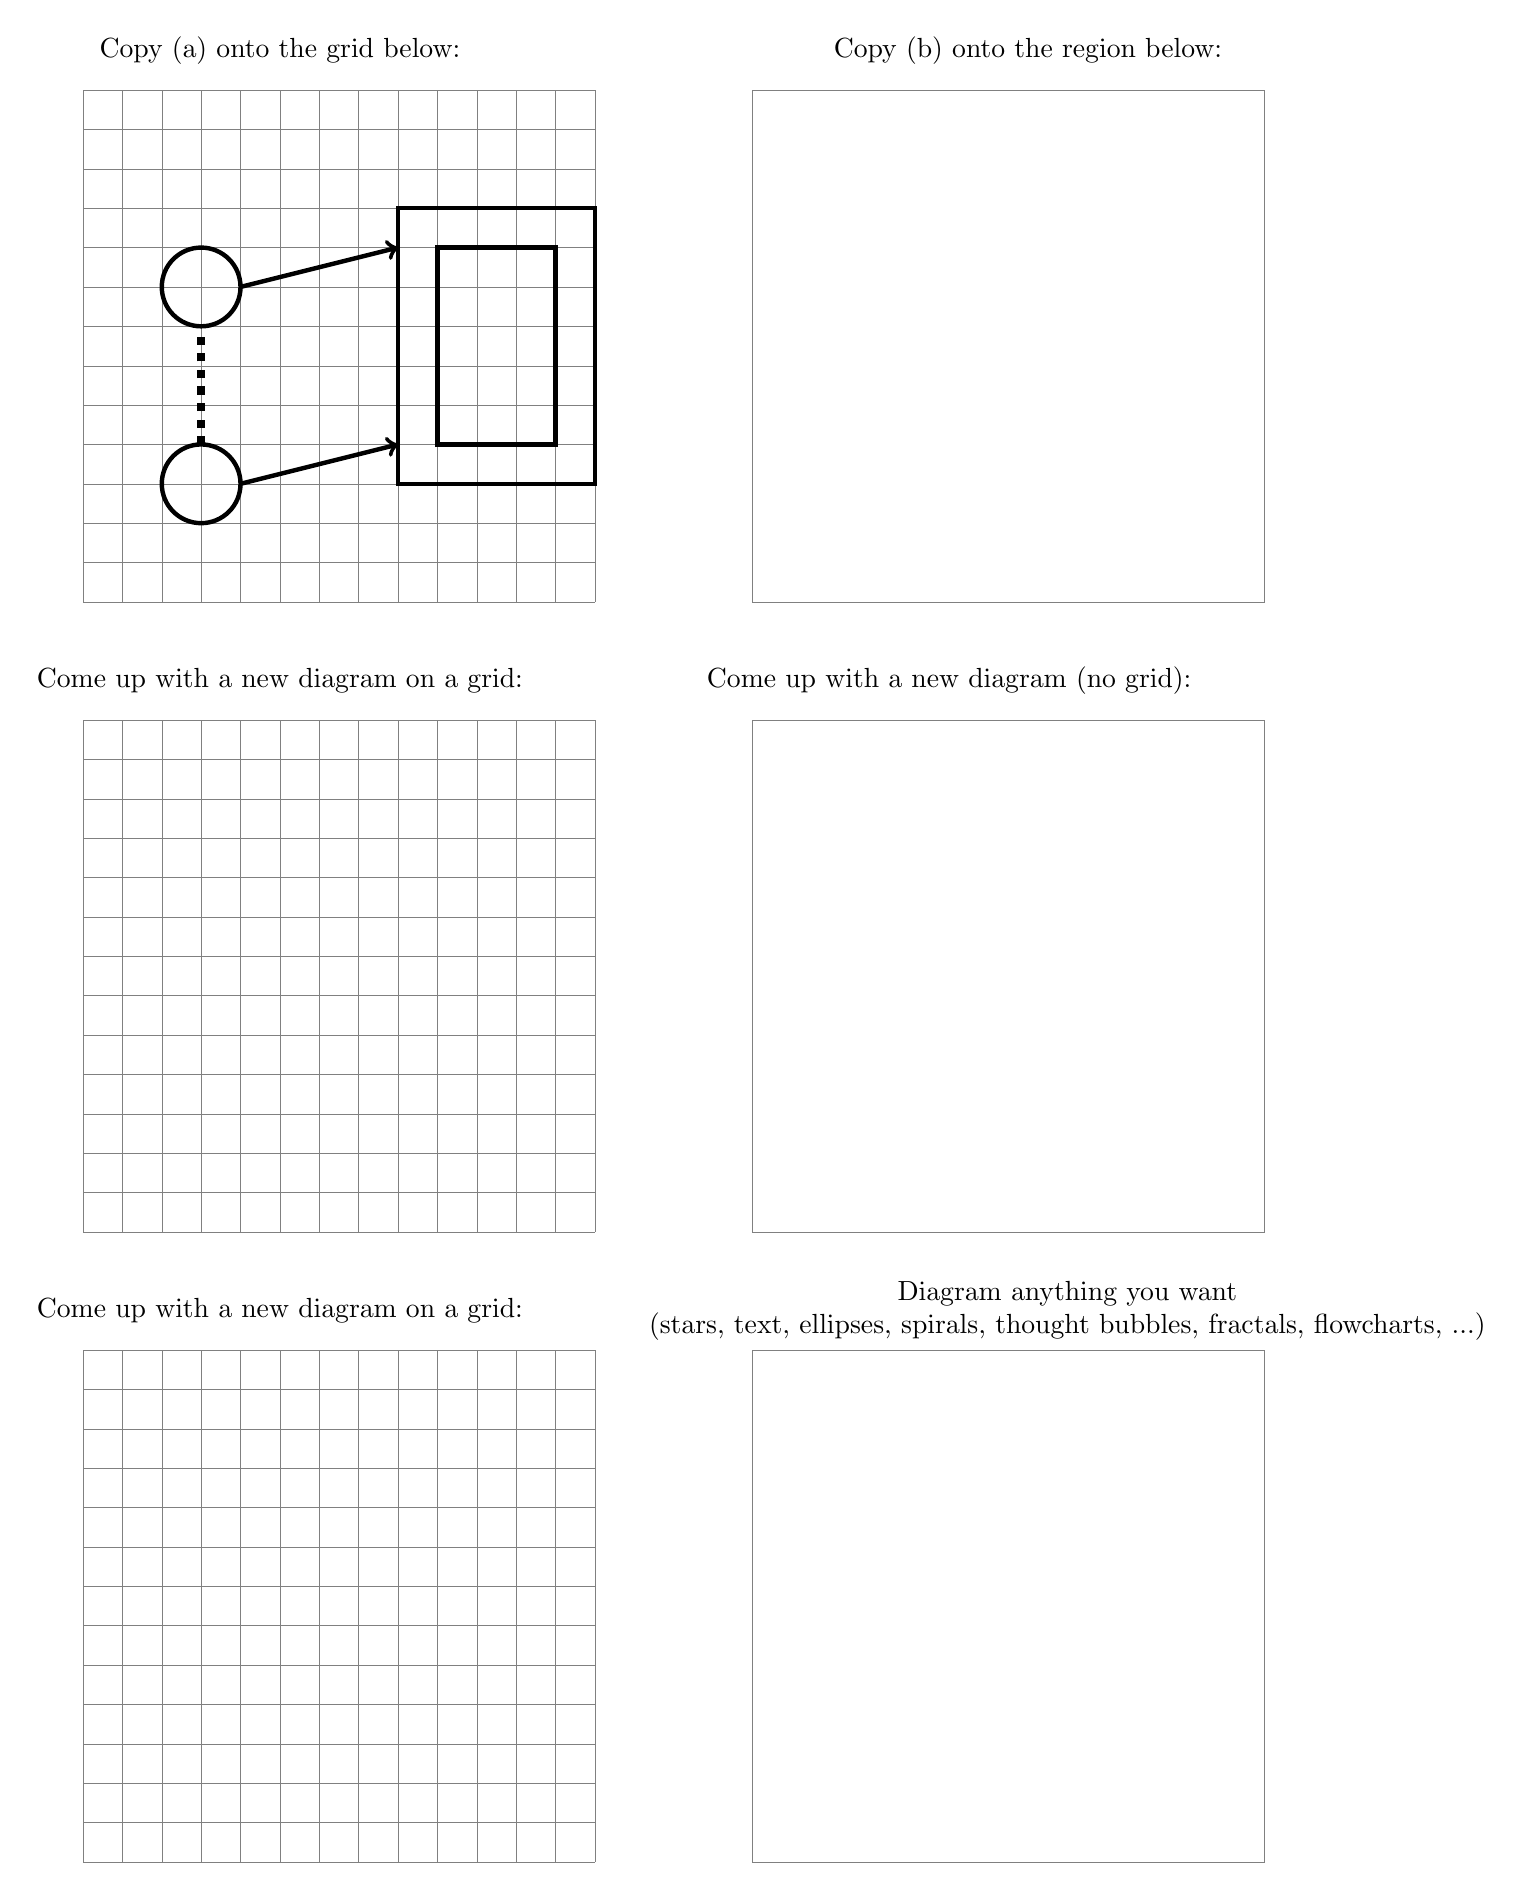
\begin{tikzpicture}[scale = 0.5]
  \node[align = right] at (5,14) {Copy (a) onto the grid below:};
  \draw[step=1cm,gray,ultra thin] (0,0) grid (13,13);
  \draw[ultra thick] (3,3) circle (1cm);
  \draw[ultra thick] (3,8) circle (1cm);
  \draw[line width = 0.1cm,dashed] (3,4) -- (3,7);
  \draw[ultra thick] (8,3) rectangle (13,10);
  \draw[ultra thick] (9,4) rectangle (12,9);
  \draw[ultra thick,-{>[scale = 1.5]}]  (4,3) -- (8,4);
  \draw[ultra thick,-{>[scale = 1.5]}]  (4,3+5) -- (8,4+5);

  \node[align = right] at (5 + 19,14) {Copy (b) onto the region below:};
    \draw[step=1cm,gray,ultra thin] (17,0) rectangle (13+17,13);

  \node[align = right] at (5,14 - 16) {Come up with a new diagram on a grid:};
  \draw[step=1cm,gray,ultra thin] (0,0-16) grid (13,13 - 16);

  \node[align = right] at (5 + 17,14 - 16) {Come up with a new diagram (no grid):};
  \draw[step=1cm,gray,ultra thin] (17,0-16) rectangle (13 + 17,13 - 16);

  \node[align = right] at (5,14 - 16 - 16) {Come up with a new diagram on a grid:};
  \draw[step=1cm,gray,ultra thin] (0,0-16 - 16) grid (13,13 - 16 - 16);

  \node[align = center] at (8 + 17,14 - 16 - 16) {Diagram anything you want\\(stars, text, ellipses, spirals, thought bubbles, fractals, flowcharts, ...)};
  \draw[step=1cm,gray,ultra thin] (17,0-16 - 16) rectangle (13 + 17,13 - 16 - 16);
\end{tikzpicture}

\pagebreak

\begin{tabular}{cc}
\textbf{(a)}  \tcbox{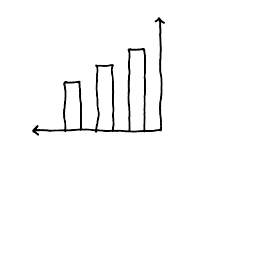
\includegraphics[width = 5cm]{figures/expert-58.png}}&  \textbf{(b)} \tcbox{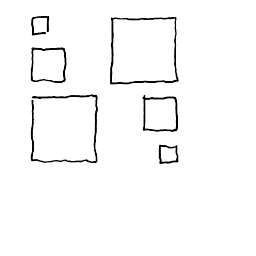
\includegraphics[width = 5cm]{figures/expert-36.png}}\\
\textbf{(c)}    \tcbox{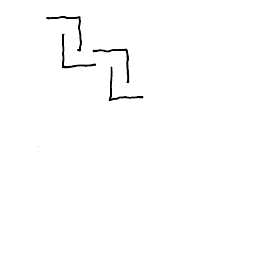
\includegraphics[width = 5cm]{figures/expert-34.png}}&\textbf{(d)}  \tcbox{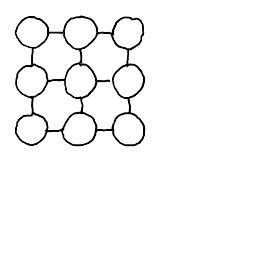
\includegraphics[width = 5cm]{figures/expert-38.png}}\\
\textbf{(e)}  \tcbox{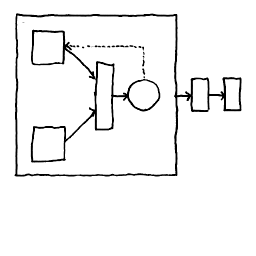
\includegraphics[width = 5cm]{figures/expert-1.png}}&  \textbf{(f)}\tcbox{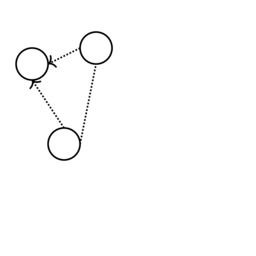
\includegraphics[width = 5cm]{figures/randomScene-33-5.png}}\\
\textbf{(g)}  \tcbox{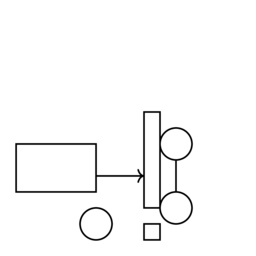
\includegraphics[width = 5cm]{figures/randomScene-58-7.png}}&  \textbf{(h)}\tcbox{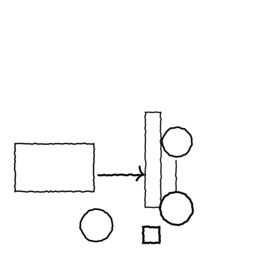
\includegraphics[width = 5cm]{figures/randomScene-58-noisy.png}}\\
\end{tabular}

\end{document}
